\documentclass[./main]{subfiles}
%
%\usepackage{amsmath, amssymb, amsthm}
%\usepackage[dvips]{graphicx}
%\usepackage{here} %画像の位置調整用
%\usepackage{okumacro} %ルビ用
%
\begin{document}

\Chapter{和算--日本の数学(大桑)}

\Section{和算の歴史}

古代から日本には数的な考え方がありました. 大和政権時代に中国・朝鮮との交易で九九を取り入れ,室町時代の勘合貿易では中国からそろばんが伝わり,商人や武士の間では生活数学が使われていたようです. 生活数学は江戸時代,貨幣社会になって計算のできる人の需要が高まったことにより,飛躍を遂げます. まず京都を中心としてそろばん塾が現れました. そこで教科書のような役割をしたのが『算用記』(1600$\sim$1620?)です. 内容は割り算,容積,土木関係,利息などの身近な数処理に関するものでした.

多くある塾の弟子たちは次第に独学で数学を学び始めます. その一人の吉田光由もそうでした. 彼は中国の数学書で独学し生活数学の本として『\ruby{塵劫記}{じんこうき}』(1627)を刊行します. その続編である『新篇塵劫記』(1641)において,巻末に答えのない問題(遺題)を12問つけました. これがきっかけとなり,数学を研究する人たちが商人に限らず増え,和算は発達を遂げるのです. このように,答えのない問題を出す伝統を遺題継承と呼んでいます.

遺題継承という伝統のほかにも,和算にはもう1つの大きな伝統があり,それが算額奉納です.絵馬に数学の問題・解法・解答を記したものを神社仏閣に奉納するというもので,江戸初期から始まっていたようです. その目的は神への感謝と,数学の実力が付くようにという祈願だとされていますが,塾の経営者や本の著者が宣伝を兼ねて算額を掲げることもあったようです. 算額は現存するだけでも全国に900枚以上存在し,そこからかなり流行したことがうかがえます. どうやら江戸時代に数学は,研究者や商人だけではなく,アマチュアの愛好家にも愛されていたようです.

発達していく和算を学ぶ者の一人に関孝和(1642?$\sim$1708)がいました. 彼は中国書を学び驚くべき業績を残しました. 例えば,円周率の小数11位までの計算,不定方程式,行列式の概念,ベルヌーイ数の発見などです. それらを可能にしたのは彼の発明した, \ruby{点竄術}{てんざんじゅつ}と呼ばれる高次方程式を解くための書法です. 彼の発明まで,数学の計算はそろばんと算木と呼ばれる棒を使って行われていたのですが,点竄術によればそれを紙上ですることができてしまいます.


\Section{和算の記法}

さて,その点竄術とはどのようなものでしょうか. それまでの計算はそろばんや算木と呼ばれる細い棒を使ってやっていたのですが,それでは複雑な式変形や多元高次方程式を解くのに難がありました.それを改善したのが点竄術です. 以下にその例を見ていきましょう.

数は次のように表します.

\begin{figure}[H]
\begin{center}
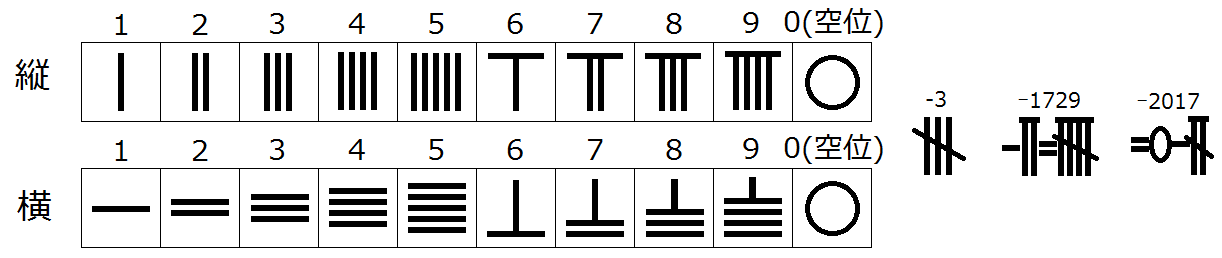
\includegraphics[width=18cm]{ookuwa0.png}
\end{center}
\end{figure}

一桁の数字には縦書きを使うのですが,2桁以上では,一,十,百,千...の位を縦,横,縦,横,...と交互に使っていきます. 123のような数字を縦書きのみで使うと何が書いてあるか分からなくなるからですね. 負の数は一の位に斜線を引いて表します.

主な式の表し方は次のようになります.

\begin{figure}[H]
\begin{center}
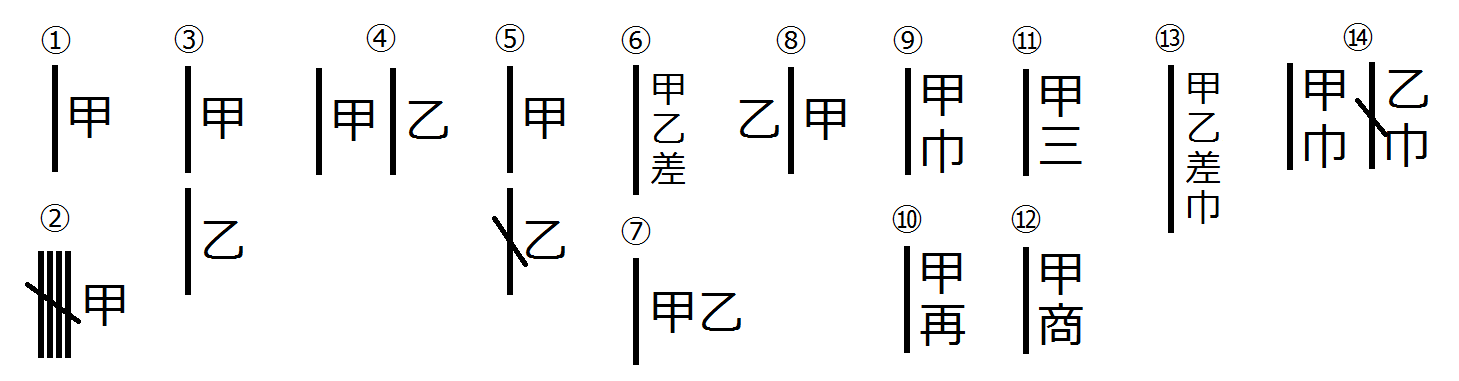
\includegraphics[width=18cm]{ookuwa1.png}
\end{center}
\end{figure}

文字としては{\sl 甲,乙,丙...}が多く使われ,他に{\sl 子,丑,寅,...天,地,人}などを使います. 問題設定によっては直角三角形の辺を{\sl 勾,股,弦},円に関する問題では直径を円径などと,そのまんま文字としてしまうこともあります. さて,$\textcircled{\scriptsize1}$は単なる甲という変数を表します. $\textcircled{\scriptsize2}$は単項式$-4 \times 甲$です. $甲+乙$は$\textcircled{\scriptsize3},\textcircled{\scriptsize4}$の2つの書き方があり,$\textcircled{\scriptsize5}$は$甲-乙$ですね. $\|甲-乙\|$は$\textcircled{\scriptsize6}$で表します. $\textcircled{\scriptsize7}$は$甲 \times 乙$,$\textcircled{\scriptsize8}$は$甲 \div 乙$です. 現在の積や分数の書き方と似ていますね. $甲^2,甲^3,甲^4,\sqrt{甲}$はそれぞれ$\textcircled{\scriptsize9},\textcircled{\scriptsize10},\textcircled{\scriptsize11},\textcircled{\scriptsize12}$で,甲四と縦に書けば5乗です. カッコの表現はないので,$(甲-乙)^2$と$甲^2-乙^2$は$\textcircled{\scriptsize13},\textcircled{\scriptsize14}$のように区別しています.例えば『算法\ruby{類聚}{るいじゅ} 巻九』では,2次方程式$c+bx-ax^2=0$の解法を次のように述べています. 

\begin{figure}[H]
\begin{center}
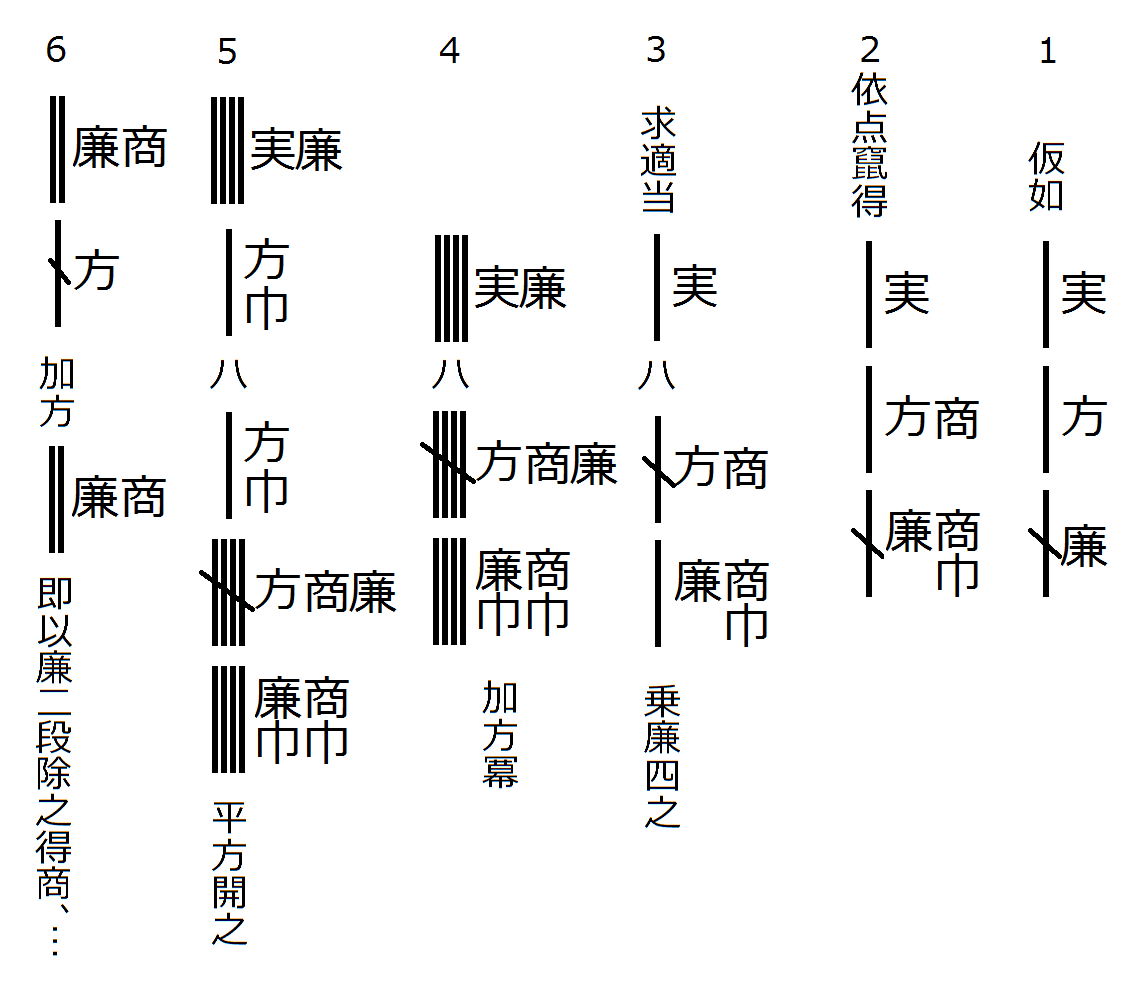
\includegraphics[width=13cm]{ookuwa2.png}
\end{center}
\end{figure}

\begin{enumerate}
\item 仮に$実,方,-廉$が与えられたとして
\item 点竄術により$実+方商-廉商^2$とする
\item $実=-方商+廉商^2$となる商を求める. $4廉$をかける.
\item $4実廉=-4方商廉+4 廉^2 商^2$. $方^2$を加える.
\item $4実廉+方^2 = 方^2 - 4方商廉 + 4 廉^2 商^2$. 開平して,
\item $2廉商-方$に方を加えて,$2廉$を除けば商を得る.
\end{enumerate}


\Section{算額の問題}

和算の伝統の一つに算額奉納があると述べました. ここでは埼玉県の\ruby{日枝}{ひえ}神社に奉納されているものを例に,算額を見てみましょう. (文章は読みやすいようにスペースを入れています.)

\begin{figure}[H]
\begin{center}
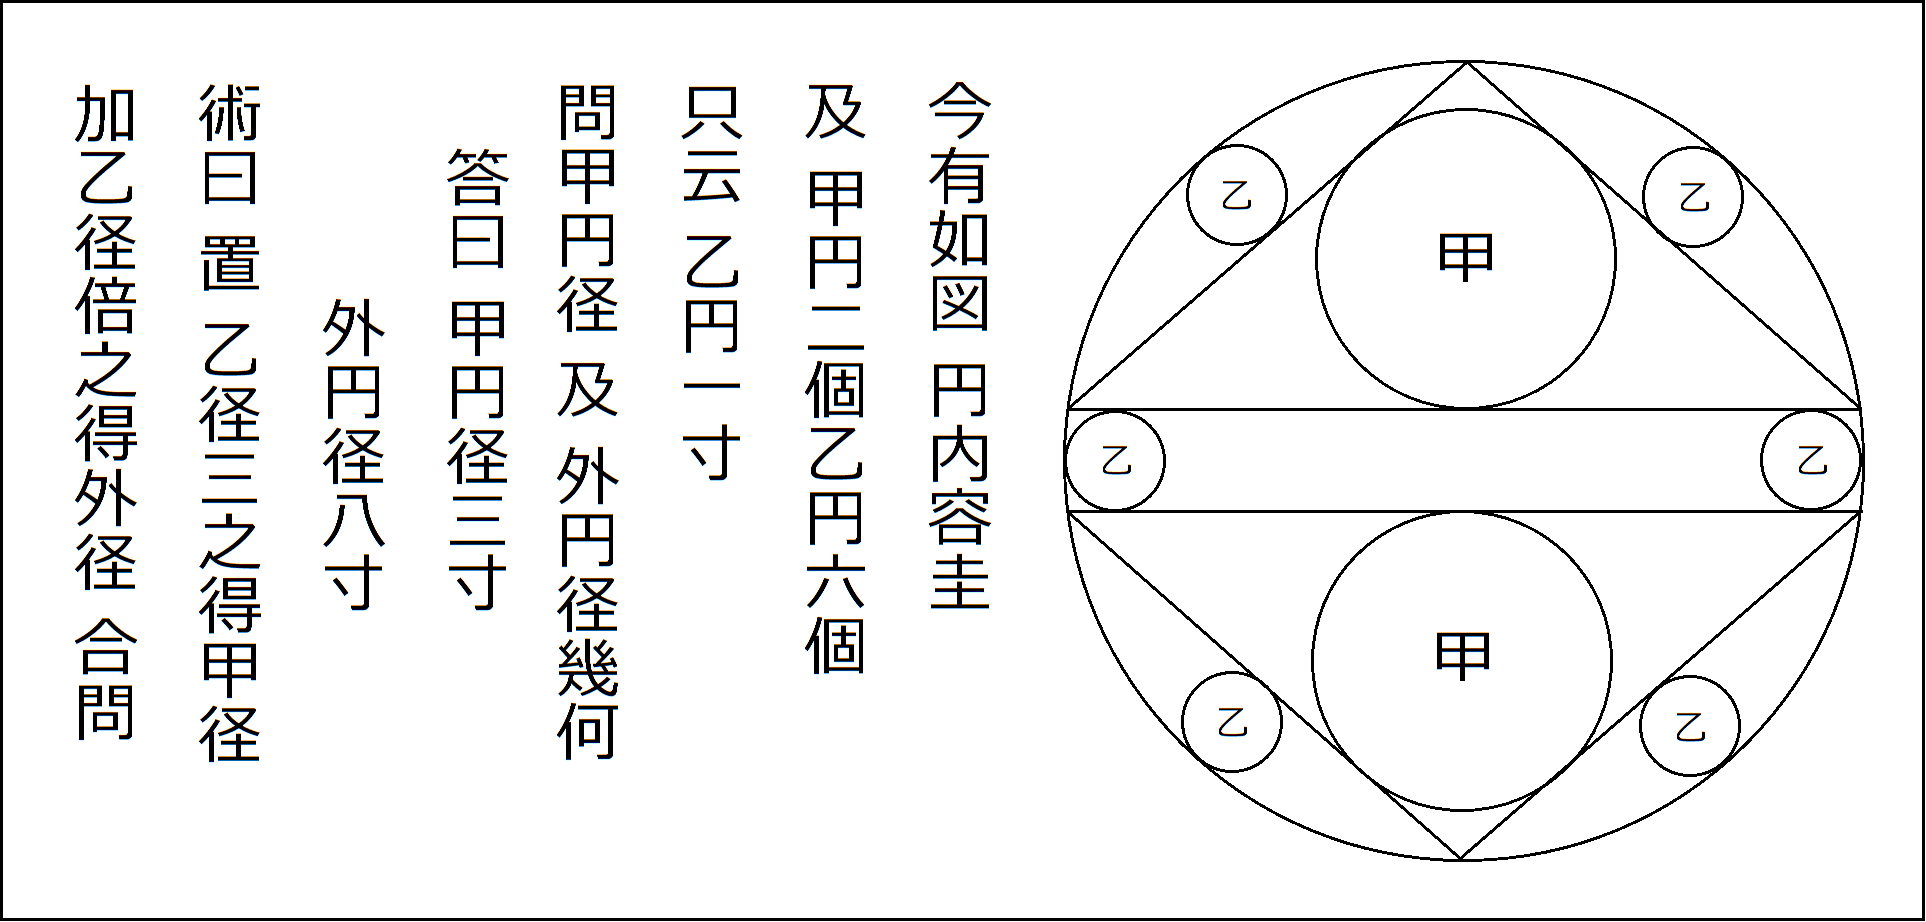
\includegraphics[width=13cm]{ookuwa3.png}
\end{center}
\end{figure}

\begin{flushleft}
[用語] \\
今有如図,術曰置:それぞれ問題文,一般解始まりの慣用句 \\
只云:数値条件始まりの慣用句 \\
圭:二等辺三角形 \\
円径:直径
\end{flushleft}

文章は三段落1.問題文, 2.答え, 3.考え方や定理(術文)に分かれています.訳してみると

\begin{enumerate}
\item 図のように外円に二等辺三角形が内接し,甲円2個と乙円6個がある. 乙円の直径を1寸とするとき,甲円の直径と外円の直径はいくらか.
\item 甲円の直径は3寸,外円の直径は3寸.
\item 乙円の直径を3倍すれば甲円の直径が得られ,それに乙円の直径を足して2倍すれば外円の直径を得る.
\end{enumerate}
という具合です. いずれも略解のようですが,それもその通り. 算額は見学者への挑戦でもあるので,詳しい解説はほとんどされません. (皆さんもぜひ手を動かして解いてみてください!)
問題の題材としては様々な図形と円がやたら接しているものが多いようです. 円に関する問題は,円周率の計算なども含めて盛んに研究され,その理論を総称して円理と呼んでいます.

最後に私が京都で見た算額を皆さんへの遺題として終わります. ありがとうございました.

\begin{figure}[H]
\begin{center}
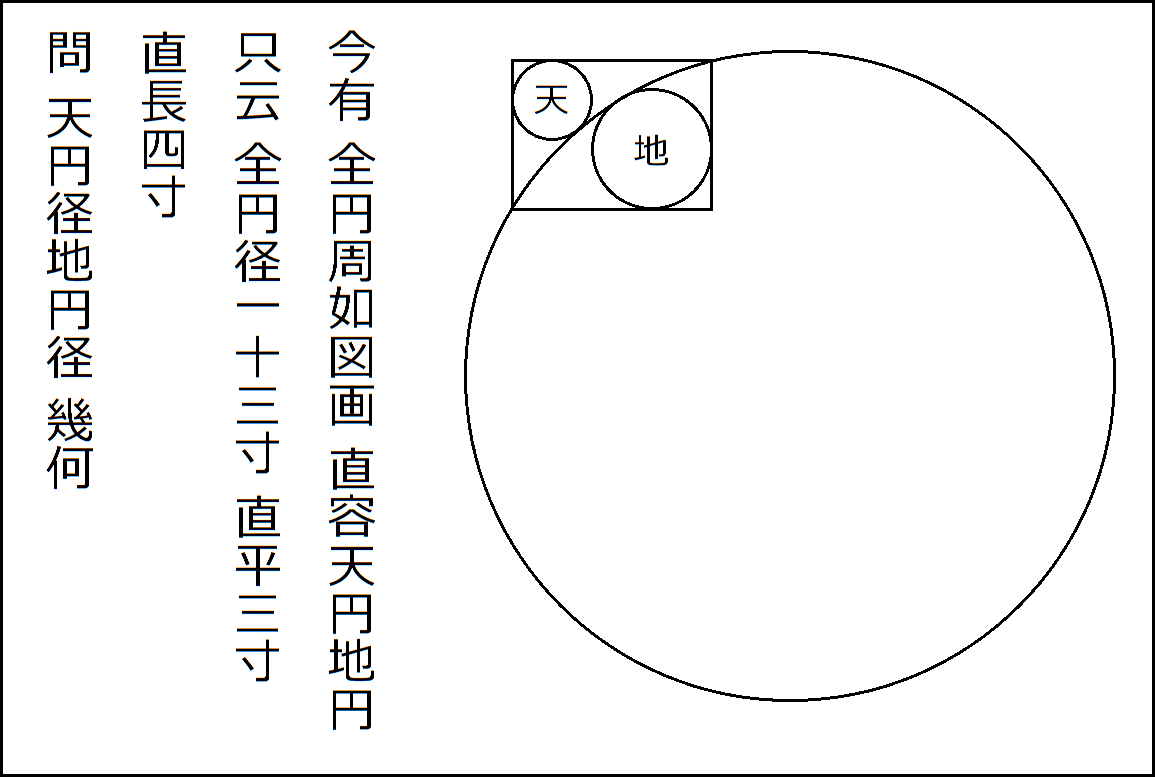
\includegraphics[width=13cm]{ookuwa4.png}
\end{center}
\end{figure}

\begin{flushleft}
[用語] \\
直:長方形 \\
容:接していること \\
直平:長方形の短い辺 \\
直長:長方形の長い辺 \\
(京都府 御香宮神社)
\end{flushleft}

\begin{thebibliography}{9}
\bibitem{oohara} 大原茂(1998)『算額を解く』さきたま出版会.
\bibitem{uegaki} 上垣渉(2006)『はじめて読む数学の歴史』ペレ出版.
\bibitem{kato} 加藤平左ェ門(1957)『和算ノ研究』日本学術振興会.
\bibitem{nishida} 山司勝紀・西田知己編(2009) 『和算の事典』 佐藤健一監修,朝倉書店.
\bibitem{kinki} 近畿数学史学会編著(1992)『近畿の算額「数学の絵馬を訪ねて」』大阪教育図書株式会社.
\end{thebibliography}

\end{document}
